\documentclass[9pt]{beamer}
\usetheme{CambridgeUS}
\usecolortheme{beaver}
\useinnertheme{rectangles}
\useoutertheme{smoothbars}

\usepackage[T1]{fontenc}
\usepackage[utf8]{inputenc}
\usepackage{lmodern}
\usepackage{textpos}

\usepackage{pdfpages}
\usepackage[english]{babel}
\usepackage{csquotes}
\usepackage{geometry}
\usepackage{graphicx}
\usepackage{subcaption}
\usepackage{hyperref}
\usepackage{url}
\usepackage{amsmath, amssymb, amsfonts}
\usepackage[super]{nth}
\usepackage{fancybox}
\usepackage{lipsum}

\usepackage{tabularx}
\usepackage{longtable}
\usepackage{booktabs}
\usepackage{array}
\usepackage{tikz}
\usetikzlibrary{arrows.meta, positioning}
\tikzset{%
  >={Latex[width=10mm, length=3mm]},
  base/.style = {rectangle, draw = black, text centered, font = \sffamily, minimum width = 1cm , minimum height = 3cm, text width = 2cm},
  ETF/.style = {base, fill = blue!80},
  AP/.style = {base, fill = blue!60},
  Investor/.style = {base, fill = red!60},
  Exchange/.style = {base, fill = lightgray},
  arrow/.style = {->, shorten >=2pt, width=10mm}
}


\usepackage[backend=biber, dateabbrev=true, citestyle=authoryear-icomp, bibstyle=authoryear-icomp, useprefix=true, language=english]{biblatex}
%\nocite{*}
\bibliography{../Bibliography/BibETF}

\setbeamertemplate{caption}[numbered]
\setbeamertemplate{bibliography item}[text]
\title[ETFs' unintended effects on stocks]{Exchange-traded funds' expansion and their unintended effects over underlying stocks}
\subtitle{Volatility, liquidity and efficiency}
\author{Gr\'egoire Pichard}
\date{\today}
\institute{HEC Lausanne (Unil)}
\subject{Master of Science in Finance (\textsc{MScF})}
%\logo{
\includegraphics[scale = 0.3]{lo_unil_hec06_bleu.eps}}

\begin{document}
\begin{frame}
  \titlepage
\end{frame}

\begin{frame}
  \frametitle{All evil rooted in one product ?}
  \shadowbox{\parbox{\textwidth}{\textbf{The Silent Road to Serfdom : Why Passive Investing is Worst Than Marxism} -- Note by I.~Fraser-Jenkins, \emph{Sanford C. Bernstein \& Co.}, 2016}}
  \begin{columns}
    \begin{column}{0.6\textwidth}
      \begin{itemize}
      \item Abstract : the shift of a growing share of capital markets towards passive, index-based investing prevents the efficient reallocation of capital from overpriced to underpriced companies. Active management and the related research generate positive externalities.
      \item Are this concern and conclusion justified ?
        \begin{itemize}
        \item What are the author's interests ? This is from the quantitative research of an asset management company, also running retail mutual funds.
        \item {In general:\\
          \begin{quote}
            Everything which is exaggerated is insignificant.\hfill{ \tiny Talleyrand}
        \end{quote}}
        \end{itemize}
      \end{itemize}
    \end{column}
    \begin{column}{0.4\textwidth}
      \begin{figure}
        \fbox{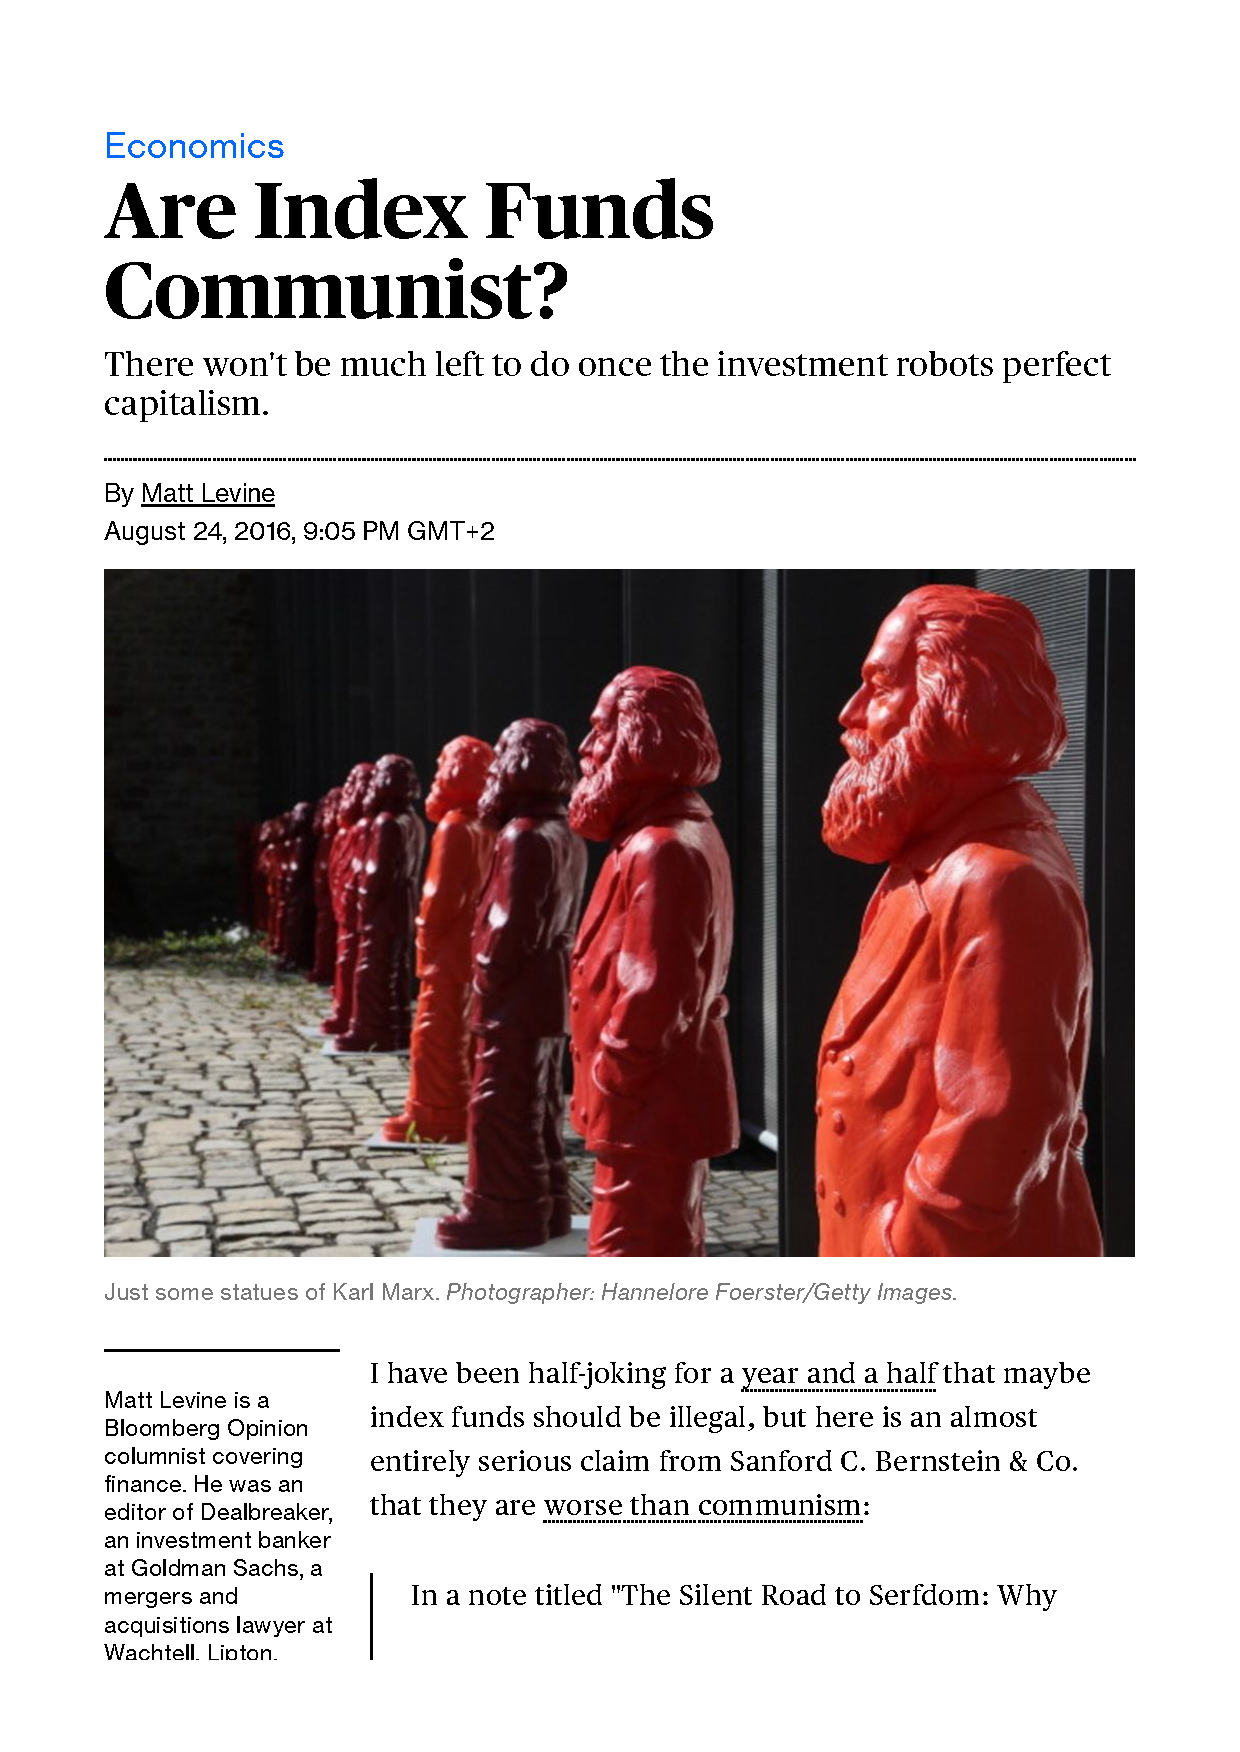
\includegraphics[page=1, width = 0.7\textwidth, height = 1.2\textwidth, keepaspectratio]{ETF_WorstThanMarxism.pdf}}
        \caption{\tiny Matt Levine, Bloomberg Opinion, 24.08.2016, available at: \url{https://www.bloomberg.com/opinion/articles/2016-08-24/are-index-funds-communist\#footnote-1472053794479}}
        \label{fig:Bloomberg_ETFMarxism}
      \end{figure}
    \end{column}
  \end{columns}
\end{frame}

\begin{frame}
  \frametitle{Research field \& focus}
  \begin{block}{General concern expressed}
    \begin{itemize}
    \item What effects are caused through index-tracking securities and \textbf{especially ETFs} on underlying securities ?
    \item Is there a new risk investors and regulators should become aware of ?
    \end{itemize}
  \end{block}
  \begin{alertblock}{Warning}
    Focusing on observable indicators of the risk and loss of efficiency is needed: choice based on existing research strategies.
  \end{alertblock}
  \begin{exampleblock}{Research questions}
    Three aspects are treated over a broad and long sample of stocks:
    \begin{enumerate}
    \item Do ETFs increase underlying stocks' volatility over the short term ?
    \item Do ETFs divert the liquidity and thus decrease it at the individual security level ?
    \item Are there signs ETFs make prices noisier, hence less efficient ? 
    \end{enumerate}
  \end{exampleblock}
\end{frame}


\begin{frame}
  \frametitle{Outline}
  \tableofcontents
\end{frame}

\section{Context}
\subsection{Exponential growth of a new fund type}
\begin{frame}
  \frametitle{Exponential growth of a new fund type}
  \only<1>{\framesubtitle{Capitalization worldwide}
    \begin{figure}
      \caption{Comparison of total stock market vs. ETF capitalization\footcite[172]{Ben-David2017}}
      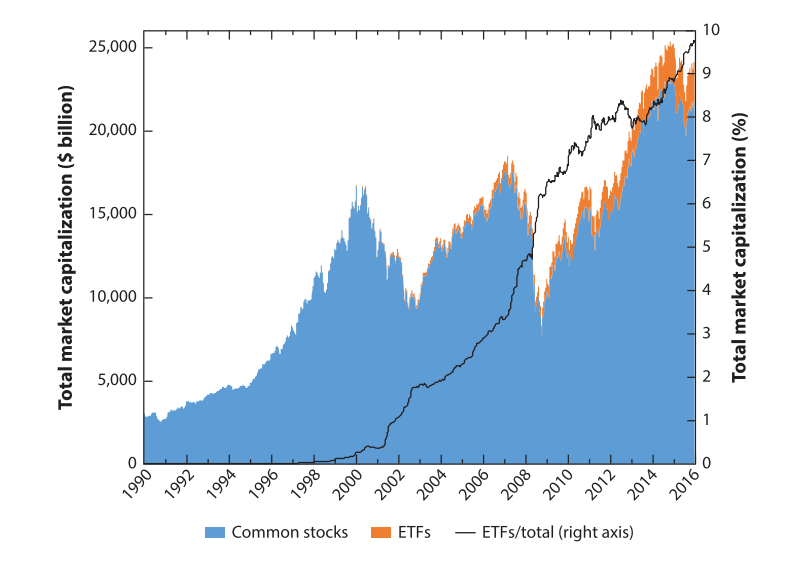
\includegraphics[width = \textwidth, height = 0.65\paperheight, keepaspectratio]{Fig1_MarketCap}
    \end{figure}
  }
  
  \only<2>{\framesubtitle{Entities listed worldwide}

  }

  \only<3>{\framesubtitle{Trading volume, share of total}
    \begin{figure}
      \caption{Comparison of total stock market vs. ETF-related daily trading volume\footcite[173]{Ben-David2017}}
      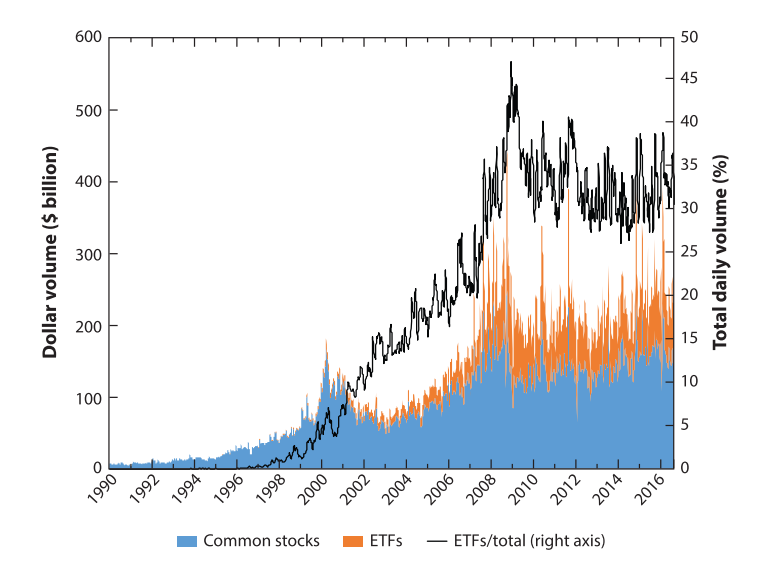
\includegraphics[width = \textwidth, height = 0.65\paperheight, keepaspectratio]{Fig2_Volume}
    \end{figure}
  }
  
\end{frame}

\subsection{Institutional aspects of ETFs}

\begin{frame}
  \frametitle{Concept and history of exchange-traded funds}
  \begin{itemize}
  \item Goal at the inception : track a value-weighted equity index using physical replication.
    \begin{itemize}
    \item First ETF ever listed : Toronto Stock Exchange Index Participation Units, introduced March 1990
    \item First ETF listed in the U.S. : State Street SPDR S\&P 500 ETF, a.k.a ``SPY'', introduced January 1993.
    \item As of June 21, 2019, SPY is the largest ETF by assets under management: USD 266~B.
    \end{itemize}
  \item A mixture of existing products:
    \begin{itemize}
    \item As (open-end) mutual funds:
      \begin{itemize}
      \item release their Net Asset Value and their holdings
      \item registered as 1940 Act investment companies $\rightarrow$ creation/redemption of shares
      \end{itemize}
    \item As index-funds : track an index built with underlying
      securities and/or derivatives and following rules defined in a
      prospectus
    \item As closed-end funds : traded throughout the day on an
      exchange
    \end{itemize}
  \end{itemize}
  \begin{alertblock}{Special features}
    \begin{itemize}
    \item the intraday NAV is spread out every 15 seconds, or more often.
    \item \textbf{standardized in-kind or cash creation/redemption process involving authorized participants' arbitrage.}
    \end{itemize}
  \end{alertblock}
\end{frame}

\begin{frame}
  \frametitle{ETF pricing mechanism and trading}
  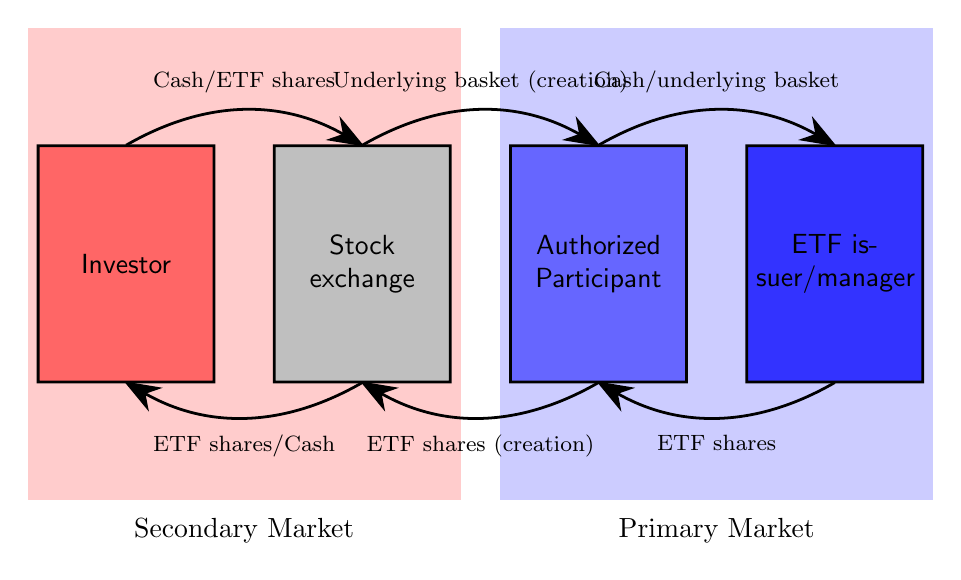
\begin{tikzpicture}[->, >={Stealth[width=3mm, length=4mm]}, auto, node distance=3cm, align = center]
    \node[base, minimum height = 6cm, minimum width = 5.5cm, fill=red!20, draw=none] at (-8.5, 0) (SecMarket) {};
    \node[base, minimum height = 6cm, minimum width = 5.5cm, fill=blue!20, right of=SecMarket, draw = none] at ([xshift=3cm] SecMarket) (PriMarket) {};
    \node[below of=PriMarket, below = 3pt] (PriMarketLabel) {Primary Market};
    \node[below of=SecMarket, below = 3pt] (SecMarketLabel) {Secondary Market};
    \begin{scope}[transparency group]
      \node at (-1,0) (ETF) [ETF] {ETF issuer/manager};
      \node (AP) [AP, left of = ETF] {Authorized Participant};
      \node (Exchange) [Exchange, left of = AP] {Stock exchange};
      \node (Investor) [Investor, left of = Exchange] {Investor};
      \draw[->] (Investor.north) to [out=30, in=150] node[above = 3pt, font=\footnotesize] {Cash/ETF shares} (Exchange.north);
      \draw[->] (Exchange.north) to [out=30, in = 150] node[above = 3pt, font=\footnotesize] {Underlying basket (creation)} (AP.north);
      \draw[->] (AP.north) to [out=30, in = 150] node[above = 3pt, font=\footnotesize] {Cash/underlying basket} (ETF.north);
      \draw[->] (ETF.south) to [in=330, out = 210] node[below = 3pt, font=\footnotesize] {ETF shares} (AP.south);
      \draw[->] (AP.south) to [in=330, out = 210] node[below = 3pt, font=\footnotesize] {ETF shares (creation)} (Exchange.south);
      \draw[->] (Exchange.south) to [in=330, out = 210] node[below = 3pt, font=\footnotesize] {ETF shares/Cash} (Investor.south);
    \end{scope}
  \end{tikzpicture}  
\end{frame}

\subsection{Evidence-based concerns expressed about ETFs}
\begin{frame}
  \frametitle{Concerns expressed about risks conveyed through ETFs}
  \begin{itemize}
  \item Liquidity : apart from idiosyncratic events, ETFs in general are very liquid thnaks to the arbitrage mechanism. E.g. \textcite{Ben-David2018} show their turnover is higher than stocks.
  \item What about underlying securities' liquidity ?
  \end{itemize}
  
\end{frame}

\begin{frame}
  \frametitle{Selection of academic contributions about ETFs' effects}
\end{frame}

\subsection{Selection of related research}
\begin{frame}
  \frametitle{Expliciting relevant research : \textcite{Ben-David2018}}
\end{frame}

\begin{frame}
  \frametitle{Expliciting relevant research : \textcite{Israeli2017}}
\end{frame}

\section{Main results}


\section{Conclusion}
\subsection{Wrap-up}

\begin{frame}
  \frametitle{Key findings}
  \begin{itemize}
  \item On average, the volatility of U.S. stocks rises with the share of their equity held by ETFs.
  \item If the mean reversion also increased because of ETFs, this volatility would be non-fundamental and the \emph{liquidity trading hypothesis} would hold.
  \item \textbf{But no significant effect has been found on U.S. variance ratios.}
  \end{itemize}
\end{frame}

\subsection{Limitations and further directions}

\begin{frame}[allowframebreaks]
  \frametitle{Likely trends in the ETF universe}
  \begin{itemize}
  \item More active bets, nicknamed \textit{passive-aggressive}
  \item Opaque holdings structures are at an advanced stage in the regulatory approval process in the U.S. (late spring 2019)
    
  \end{itemize}
  \begin{block}{The Precidian model}
    \shadowbox{\parbox{0.9\textwidth}{\textbf{An ETF That Hides Its Secret Sauce Is Poised for Regulator's Nod} -- Bloomberg News, April 8, 2019.\footnote{Available at \url{https://www.bloomberg.com/news/articles/2019-04-08/an-etf-that-hides-its-secret-sauce-is-poised-for-regulator-s-nod}}}}
    \begin{itemize}
    \item Positive signs that the Securities and Exchange Commission will allow the design.
    \item Trading permission is the next decision needed before the product is issued.
    \item Disagreement at the SEC and skepticism from some analysts regarding appeal to investors; reality check needed and \textit{evidence so far has shown that \textcolor{red}{awareness about ETFs can take time}}.
    \end{itemize}
    
  \end{block}
  
\end{frame}


\begin{frame}
  \frametitle{Bibliography}
  \printbibliography
\end{frame}
\appendix
\section{Regression results}
\subsection{Volatility}
\subsubsection{United States}
\begin{frame}[allowframebreaks, t]
  \frametitle{Volatility -- U.S. sample}
  \centering
    {\small\tabcolsep=3pt
\begin{longtable}{>{\bfseries}lcccc}
\multicolumn{5}{r}{\textit{Continued from previous page}}\\
\toprule
& \textbf{Baseline}  & \textbf{Controls + Vol. lags} & \textbf{Inst. o'ship controls} & \textbf{Standardized}  \\
\midrule
\endhead
\caption{U.S. Sample : Exchange-Traded Fund aggregate ownership share and the volatility of underlying securities' daily returns}\\
\label{tab:Volatility:US:Comp}\\
\toprule
& \textbf{Baseline}  & \textbf{Controls +lags} & \textbf{O'ship controls} & \textbf{Standardized}  \\
\midrule
\endfirsthead
\bottomrule
\multicolumn{5}{r}{\textit{Continues on next page}}\\
\endfoot
\bottomrule
\endlastfoot
Intercept                         &       0.2964       &             0.0488            &             0.0494             &        -0.0154         \\
         &      (22.268)      &            (7.1942)           &            (7.2977)            &       (-0.4273)        \\
$\mathbf{PctETF}_{t-1}$            &       0.2470       &             0.0385            &             0.0395             &         0.0081         \\
        &      (8.2542)      &            (5.9800)           &            (6.2940)            &        (6.8269)        \\
$\log(\mathbf{MarketCap}_{t-1})$    &      -0.0127       &            -0.0018            &            -0.0018             &        -0.0102         \\
         &     (-20.751)      &           (-5.8479)           &           (-5.9701)            &       (-6.1991)        \\
$1/\mathbf{Close}_{t-1}$                    &       0.0988       &             0.0251            &             0.0251             &         0.1452         \\
            &      (10.972)      &            (7.7261)           &            (7.7792)            &        (7.9151)        \\
$\left(BE/ME\right)_{t-1}$           &     5.552e-07      &           7.393e-07           &           1.038e-06            &       5.019e-06        \\
            &      (2.3023)      &            (4.1534)           &            (8.5166)            &        (5.3019)        \\
$\mathbf{Past 12 to 1M ret.}_{t-1}$               &      -0.0003       &            -0.0004            &            -0.0004             &        -0.0024   \\
&     (-0.6844)      &           (-1.8758)           &           (-1.8564)            &       (-1.8927)        \\
$\mathbf{AmihudRatio}_{t-1}$                 &                    &             3.4590            &             3.4611             &         19.952         \\
        &                    &            (2.7034)           &            (2.7029)            &        (2.7038)        \\
$\mathbf{BidAskSpread}_{t-1}$             &                    &             0.1750            &             0.1748             &         1.0060         \\
 &                    &            (4.5505)           &            (4.5446)            &        (4.5471)        \\
$\mathbf{G.Profit.}_{t-1}$          &                    &            -0.0005            &            -0.0005             &        -0.0028         \\
            &                    &           (-2.6218)           &           (-2.6334)            &       (-2.6197)        \\
$\mathbf{Volatility}_{t-1}$                  &                    &             0.1377            &             0.1378             &         0.1376         \\
       &                    &            (6.7584)           &            (6.7701)            &        (6.7630)        \\
$\mathbf{Volatility}_{t-2}$                  &                    &             0.1605            &             0.1604             &         0.1603         \\
                &                    &            (16.002)           &            (15.972)            &        (15.949)        \\
$\mathbf{Volatility}_{t-3}$                  &                    &             0.1230            &             0.1229             &         0.1229         \\
                            &                    &            (13.390)           &            (13.402)            &        (13.403)        \\
$\mathbf{Volatility}_{t-4}$                  &                    &             0.0819            &             0.0818             &         0.0817         \\
                 &                    &            (9.8851)           &            (9.8688)            &        (9.8756)        \\
$\mathbf{PctOtherMutual}_{t-1}$    &                    &                               &            -0.0003             &        -0.0016         \\
                       &                    &                               &           (-2.5676)            &       (-1.1497)        \\
$\mathbf{PctPension}_{t-1}$        &                    &                               &             1.0330             &         0.0015         \\
                               &                    &                               &            (3.4034)            &        (3.6451)        \\
$\mathbf{PctHedge}_{t-1}$          &                    &                               &            -0.0284             &       9.023e-05        \\
                           &                    &                               &           (-3.2527)            &        (0.4613)        \\
\midrule
Effects                           &       Entity       &             Entity            &             Entity             &         Entity         \\
& Time &  Time  &  Time &  Time\\
\bottomrule
\pagebreak
\toprule
& \textbf{Baseline}  & \textbf{Controls +lags} & \textbf{O'ship controls} & \textbf{Standardized}  \\
\midrule
Dep. Variable                     &     Volatility     &           Volatility          &           Volatility           &       Volatility       \\
Estimator                         &      PanelOLS      &            PanelOLS           &            PanelOLS            &        PanelOLS        \\
No. Observations                  &       413304       &             297405            &             297399             &         297247         \\
Cov. Est.                         &   Driscoll-Kraay   &         Driscoll-Kraay        &         Driscoll-Kraay         &     Driscoll-Kraay     \\
$R^{2}$                         &       0.0545       &             0.1592            &             0.1593             &         0.1594         \\
$R^{2}$ (Within)                &       0.0565       &             0.1353            &             0.1351             &         0.1348         \\
$R^{2}$ (Between)               &       0.2009       &             0.7626            &             0.7625             &         0.7616         \\
$R^{2}$ (Overall)               &       0.1515       &             0.2716            &             0.2715             &         0.2710         \\
F-statistic                       &       4717.9       &             4643.9            &             3718.4             &         3718.6         \\
P-value (F-stat)                  &       0.0000       &             0.0000            &             0.0000             &         0.0000         \\
\bottomrule
\end{longtable}
}

\end{frame}
\subsubsection{International}
\begin{frame}[allowframebreaks]
  \frametitle{Volatility -- International sample}
\end{frame}
\subsection{Liquidity}
\subsubsection{United States}
\begin{frame}[allowframebreaks]
  \frametitle{Liquidity -- U.S. sample}
\end{frame}
\subsubsection{International}
\begin{frame}[allowframebreaks]
  \frametitle{Liquidity -- International sample}
\end{frame}
\subsection{Efficiency}
\subsubsection{United States}
\begin{frame}[allowframebreaks]
  \frametitle{Efficiency -- U.S. sample}
\end{frame}
\subsubsection{International}
\begin{frame}[allowframebreaks]
  \frametitle{Efficiency -- International sample}
\end{frame}
\end{document}
